% Librarian demo in MuJoCo: what is simulated, what is plotted, when the skin helps.
% Build: cd docs/report_sim && pdflatex librarian_sim.tex && pdflatex librarian_sim.tex
% Figures: python scripts_sim/make_report_figures.py (needs a run, the ablation and the demo video).
\documentclass[10pt,twocolumn]{article}
\usepackage[letterpaper,margin=0.55in,top=0.55in,bottom=0.6in,columnsep=0.22in]{geometry}
\usepackage{mathptmx}
\usepackage[T1]{fontenc}
\usepackage{microtype,graphicx,booktabs,tikz,amsmath,enumitem,tabularx}
\usepackage[font=footnotesize,labelfont=bf,skip=3pt]{caption}
\usepackage[compact]{titlesec}
\usepackage[hidelinks]{hyperref}
\usetikzlibrary{patterns,decorations.pathmorphing,arrows.meta}
\titleformat*{\section}{\normalsize\bfseries}
\titleformat*{\subsection}{\small\bfseries\itshape}
\titlespacing*{\section}{0pt}{5pt}{2pt}
\titlespacing*{\subsection}{0pt}{3pt}{1pt}
\setlist{nosep,leftmargin=*}
\setlength{\parskip}{0pt}
\setlength{\textfloatsep}{6pt}
\setlength{\floatsep}{5pt}
\setlength{\abovedisplayskip}{3pt}\setlength{\belowdisplayskip}{3pt}
\setlength{\abovedisplayshortskip}{2pt}\setlength{\belowdisplayshortskip}{2pt}
\newcommand{\code}[1]{\texttt{\small #1}}

\title{\vspace{-4mm}\large\textbf{The librarian demo in MuJoCo: how contact force and deformation are simulated,\\
what the skin panel plots, and when the skin helps}\vspace{-2mm}}
\author{\small Dohyun, Jihoon \quad (AM/ME/CE 295, Caltech) \quad --- simulation notes, \today}
\date{\vspace{-7mm}}

\begin{document}
\maketitle

%==============================================================================
\section{The demo, end to end}
A UR10e with a Robotiq 2F-140 whose fingertips are our blades (\code{gripper\_dohyun\_v1}, a 0.5\,mm PDMS layer on
each flat face) takes a 40\,mm book out of shelf A by approaching horizontally and shelves it in a 70\,mm slot of
shelf B, turned 45\textdegree{} toward the robot (Fig.~\ref{fig:story}). The task script uses only the
\code{python-urx} calls of the real robot (\code{movel}, \code{speedl}, \code{get\_tcp\_force},
\code{gripper\_action}, \ldots), so the same file drives the hardware. The video
(\code{docs/media/librarian\_demo.mp4}) has three synchronised panels: \emph{left}, what the skin feels
(Sec.~\ref{sec:plots}); \emph{centre}, MuJoCo rendered with the Filament physically based renderer plus a
close-up that follows the tool, with arrows for the squeeze (blue) and friction (orange) on the book and the arm's
wrench (green); \emph{right}, the wrist camera and a urx console (joint angles, TCP pose and wrench, Robotiq
registers, the last commands).

\begin{figure}[t]\centering
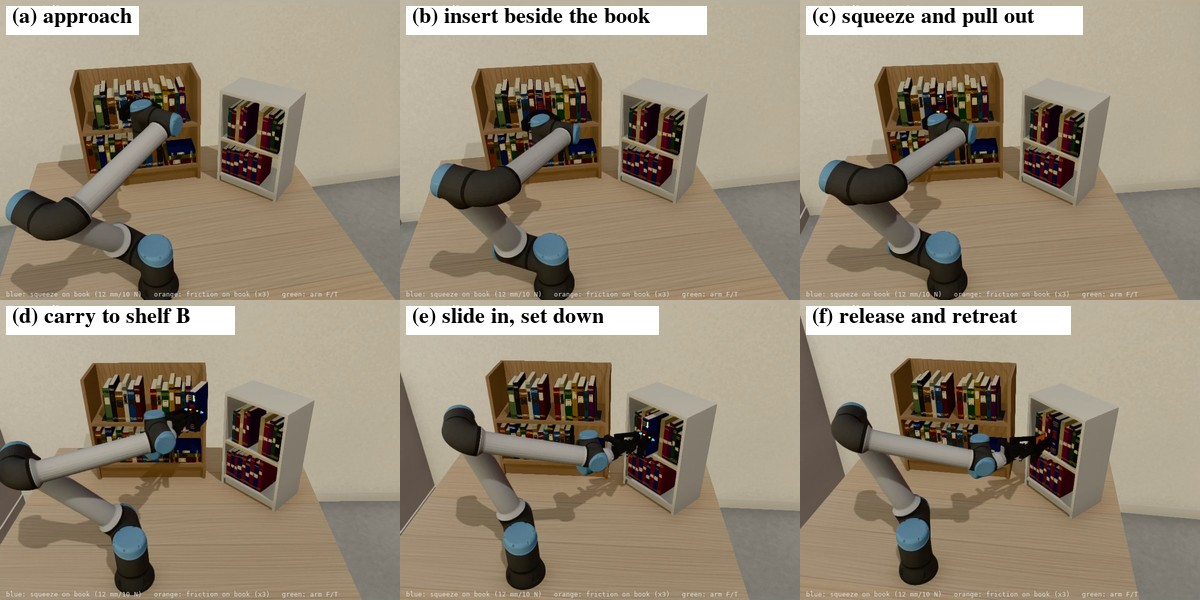
\includegraphics[width=\columnwidth]{fig_storyboard.jpg}
\caption{Key frames of the run (MuJoCo, Filament renderer). The blades slide into the 10\,mm gaps beside the
book (b); a 50\,Hz controller squeezes, pulls the book out 21\,cm and lifts it 8\,cm (c); urx moves carry it to
shelf B (d), slide it into the slot and set it down on a force threshold (e).}
\label{fig:story}
\end{figure}

%==============================================================================
\section{How MuJoCo produces force and displacement}
\subsection{Rigid bodies, joints and one step}
The state is the generalised position $q$ (joint angles, the pose of every free book, and the PDMS cells'
displacements, Sec.~\ref{sec:pdms}) and velocity $v$. Each step of $h=0.5$\,ms solves
\begin{equation}
M(q)\,\dot v + c(q,v) = \tau + J(q)^{\top} f ,
\label{eq:eom}
\end{equation}
with $M$ the mass matrix, $c$ Coriolis/gravity, $\tau$ actuator and passive (spring, damper) forces, and $f$ the
\emph{constraint forces}: contacts, the gripper's linkage (joint equalities) and joint limits, mapped by their
Jacobian $J$ \cite{todorov2012mujoco}. Bodies are rigid: a book or a blade never strains. A
\textbf{displacement} in MuJoCo is therefore a change of $q$ --- a body pose, a joint angle, or a degree of freedom
we add on purpose to represent deformation (the PDMS layer).

\subsection{Contact forces}
Collision detection finds, for each pair of touching geoms, a contact frame (normal $n$, tangents $t_1,t_2$) and
the signed distance $r$ ($r<0$: overlap). The contact force $f=(f_n,f_{t1},f_{t2})$ must lie in the friction cone
$\|f_t\|\le\mu f_n$, $f_n\ge 0$ (elliptic). MuJoCo computes all constraint forces of the step at once from a
convex problem (Gauss's principle with \emph{soft} constraints \cite{todorov2014convex,mujocodocs}): the forces make
each constraint's acceleration $a=J\dot v$ approach a reference
\begin{equation}
a^{\rm ref} = -b\,\dot r - k\,r ,
\label{eq:aref}
\end{equation}
a spring--damper set by \code{solref} (time constant, damping ratio), mixed with the unconstrained acceleration by
an impedance $d\in(0,1)$ from \code{solimp} (regulariser $R=\tfrac{1-d}{d}\hat A$). Hence (i) contact forces are
genuine forces in N: they balance gravity and actuation in Eq.~\eqref{eq:eom} and obey action--reaction;
(ii) contacts are slightly soft: at rest a small overlap $r$ remains, about $\tfrac{1-d}{d}$ of the unresisted
acceleration divided by $k$; (iii) friction is regularised: there is no static/kinetic difference and a sustained
tangential load produces a slow creep (we keep it below 0.05\,mm/s with a stiff friction-to-normal impedance ratio,
\code{impratio}\,=\,100; Sec.~\ref{sec:lim}).
Sensors are computed from the same solution: the UR10e's built-in wrist force/torque sensor is the wrench the
flange transmits (MuJoCo \code{force}/\code{torque} sensors), minus the declared payload weight, as UR reports it.

\subsection{The PDMS layer as a deformable body}\label{sec:pdms}
MuJoCo has two ways to model deformable material \cite{mujocodocs}: \emph{flex} elements (vertices are point
masses; triangles or tetrahedra carry a Saint Venant--Kirchhoff finite-element elasticity with Young's modulus
$E$ and Poisson's ratio $\nu$), and \emph{lumped} models (rigid bodies joined by elastic joints or tendons). Our
layer is $t=0.5$\,mm thick over $51\times71$\,mm. We first built it as a 3D flex ($6\times8\times2$ vertices): on a
fixed plate its shear stiffness was within 17\% of the analytical value, but bolted to the moving finger its thin
elements (aspect ratio 20:1 and more) made MuJoCo's effective-inertia solve ill-conditioned (contact and elastic
forces no longer balanced). We therefore use the \emph{thin-layer limit} of linear elasticity, which is exact when $t$ is much
smaller than the loaded area \cite{johnson1985,shull2002}: each column of PDMS deforms under its own traction only
(a Winkler foundation). The layer is split into $5\times7$ cells of area $A=10.2\times10.1$\,mm$^2$; each cell is a
point mass bonded to the blade by three slide joints (compression $u_z$, shear $u_x,u_y$) with
\begin{equation}
k_n=\frac{E(1-\nu)}{(1+\nu)(1-2\nu)}\frac{A}{t},\qquad k_s=\frac{E}{2(1+\nu)}\frac{A}{t},
\label{eq:k}
\end{equation}
(confined compression and shear of the column) and Kelvin--Voigt damping $\tau_d k$
(Fig.~\ref{fig:layer}). With the placeholders $E=1$\,MPa (Sylgard-184-like \cite{johnston2014}), $\nu=0.45$,
$\tau_d=1$\,ms: $k_n=7.8\times10^5$ and $k_s=7.1\times10^4$\,N/m per cell. A 50\,mg cell on such a spring
oscillates at $\omega\approx1.3\times10^5$\,rad/s, so an explicit integrator would need $h<2/\omega\approx16\,\mu$s.
MuJoCo's \code{discrete} integrator is implicit in position: it folds the stiffness into the effective inertia
$\hat M=M+hD+h^2K$ and is stable at 0.5\,ms; the layer then responds quasi-statically (in $\sim$1\,ms), which is all
a grasp needs. Each cell touches the object at one point (a flat ellipsoid filling the cell); that contact's own
softness stands for the object's surface (a book cover), not for the PDMS.

\begin{figure}[t]\centering
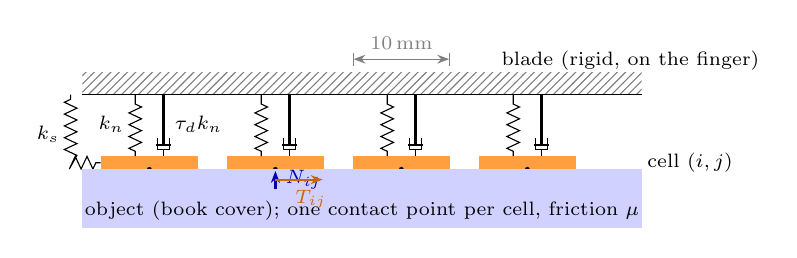
\begin{tikzpicture}[x=1cm,y=1cm,>={Stealth[length=1.5mm]},
  spring/.style={decorate,decoration={zigzag,segment length=1.5mm,amplitude=0.8mm,pre length=0.6mm,post length=0.6mm}}]
  \fill[pattern=north east lines,pattern color=black!50] (-0.1,1.50) rectangle (7.0,1.78);
  \draw (-0.1,1.50) -- (7.0,1.50);
  \node[font=\scriptsize,anchor=west] at (5.1,1.93) {blade (rigid, on the finger)};
  \foreach \i in {0,...,3} {
    \pgfmathsetmacro{\x}{0.75+1.6*\i}
    \fill[orange!75] (\x-0.62,0.55) rectangle (\x+0.62,0.72);
    \draw[spring] (\x-0.18,0.72) -- (\x-0.18,1.50);
    \draw[thick] (\x+0.18,0.86) -- (\x+0.18,1.50); \draw (\x+0.08,0.86) -- (\x+0.28,0.86);
    \draw (\x+0.10,0.80) -- (\x+0.10,0.95) (\x+0.26,0.80) -- (\x+0.26,0.95) (\x+0.10,0.80) -- (\x+0.26,0.80);
    \draw (\x+0.18,0.72) -- (\x+0.18,0.80);
    \fill (\x,0.55) circle (0.9pt);
  }
  \draw[spring] (0.13,0.635) -- (-0.25,0.635) -- (-0.25,1.50);
  \node[font=\scriptsize,anchor=east] at (0.55,1.12) {$k_n$};
  \node[font=\scriptsize,anchor=west] at (0.95,1.12) {$\tau_d k_n$};
  \node[font=\scriptsize,anchor=east] at (-0.27,1.0) {$k_s$};
  \node[font=\scriptsize,anchor=west] at (6.95,0.64) {cell $(i,j)$};
  \fill[blue!18] (-0.1,-0.20) rectangle (7.0,0.55);
  \node[font=\scriptsize] at (3.45,0.02) {object (book cover); one contact point per cell, friction $\mu$};
  \draw[->,thick,blue!70!black] (2.35,0.30) -- node[right,font=\scriptsize]{$N_{ij}$} (2.35,0.53);
  \draw[->,thick,orange!80!black] (2.35,0.42) -- node[below,font=\scriptsize,pos=0.75]{$T_{ij}$} (2.95,0.42);
  \draw[|<->|,gray] (3.95-0.62,1.95) -- node[above,font=\scriptsize]{10\,mm} (3.95+0.62,1.95);
\end{tikzpicture}
\caption{The PDMS layer as simulated: $5\times7$ columns of PDMS, each a point mass on three elastic slide joints
(normal shown; two shear springs act along the face) bonded to the blade. Contact forces $N_{ij},T_{ij}$ come from
MuJoCo's contact solver; the deformation $u_{ij}$ is the cells' joint positions.}
\label{fig:layer}
\end{figure}

%==============================================================================
\section{What the skin panel plots}\label{sec:plots}
Table~\ref{tab:plots} separates what the physics model computes from what we \emph{assume} about a sensor that is
not characterised yet. The panel shows, per blade, a map of the contact force per cell (colour: normal $N_{ij}$;
arrows: shear $T_{ij}$), a map of the layer's deformation (colour: compression; arrows: shear displacement), and
time series of $N=\sum N_{ij}$, $|T|=|\sum T_{ij}|$, the margin $q$ with the Robotiq force setting, and the arm's
wrench with the book's slip. In the quasi-static limit the cell's elastic force equals its contact force
($k_s u_{xy}=T_{ij}$, $k_n u_z=N_{ij}$, checked to within 2\% in our tests), so the two maps carry the same
information here; a real sensor may report either, or strain, through its own unknown transfer function. The
margin of each blade treats its contact patch as a whole, using an elliptical limit surface for sliding and
twisting \cite{goyal1991,howe1996}:
\begin{equation}
q = 1-\sqrt{\left(\frac{|T|}{\mu N}\right)^{2}+\left(\frac{|M|}{\mu N\rho}\right)^{2}},\quad
\rho=\tfrac23\sqrt{A_c/\pi},
\label{eq:q}
\end{equation}
where $M=\sum (r_{ij}-c)\times T_{ij}$ is the twist of the shear field about the centre of pressure $c$ and $A_c$
the loaded area ($\rho$ of a uniformly loaded disc). $q=1$: no load; $q\le0$: the patch slides or twists. The
grasp margin is the weaker blade, $Q=\min(q_L,q_R)$. Without the twist term the book rotated out of the grasp: it
is held near its spine, 65\,mm from its centre of mass.

\begin{table}[t]\centering\footnotesize
\setlength{\tabcolsep}{2.5pt}
\begin{tabularx}{\columnwidth}{@{}l>{\raggedright\arraybackslash}Xl@{}}
\toprule
plotted quantity & how it is computed & status \\
\midrule
$N_{ij}$, $T_{ij}$ per cell & sum of the solver's contact forces on cell $(i,j)$, in the PDMS frame & model physics \\
deformation $u_{ij}$ & the cell's joint positions (Eq.~\ref{eq:k}) & placeholder $E,\nu$ \\
$N$, $|T|$, CoP, $M$ & sums and moments over the cells & derived \\
margin $q$, $Q$ & Eq.~\eqref{eq:q} & assumes $\mu=1$ \\
5$\times$7 cells, 20\,Hz & grid of the model; 50\,ms frame averages & assumed sensor \\
noise, drift, hysteresis & none & not modelled \\
arm F/T & flange wrench $-$ payload weight & as UR10e \\
slip, rotation & book pose relative to the TCP since grasp & sim only \\
\bottomrule
\end{tabularx}
\caption{The skin panel, separated into what MuJoCo computes and what is assumed about the (uncharacterised)
sensor. ``Model physics'': exact within the model, whose material values are placeholders.}
\label{tab:plots}
\end{table}

\begin{figure}[t]\centering
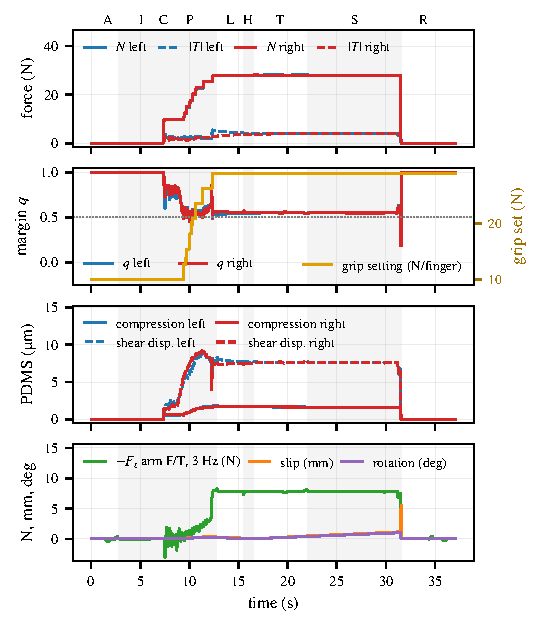
\includegraphics[width=\columnwidth]{fig_run.pdf}
\caption{The demo run (0.8\,kg book, $\mu=1$, skin controller). Letters mark the phases: approach, insert, close, pull,
lift, hold, carry (T), shelve (S), retreat. The controller raised the grip in steps until $q$ settled at 0.55, just
above $q^\star=0.5$: 28\,N per blade ($|T|=3.9$\,N). Holding, the PDMS compressed 1.7\,$\mu$m and sheared up to
7.6\,$\mu$m (a twist pattern: the book hangs 65\,mm off the patch); the wrist F/T read the 7.8\,N book. The book
slipped 0.5\,mm and 0.4\textdegree{} before set-down and landed 2\,mm from the slot centre; neighbours moved
0.03\,mm.}
\label{fig:run}
\end{figure}

%==============================================================================
\section{Control, and who decides what}
\textbf{Arm.} Every urx call becomes joint targets for MuJoCo position servos with gravity compensation (as the
UR controller does): \code{movej} by trapezoidal joint profiles; \code{movel} by a straight TCP line (and an
angle--axis rotation) converted every 2\,ms with damped least-squares inverse kinematics
$\Delta q=J^\top(JJ^\top+\lambda^2 I)^{-1}e$ \cite{wampler1986}; \code{speedl} by integrating a TCP twist through
the same IK. The UR10e's published DH parameters are used, so poses match the real controller.
\textbf{Gripper.} Robotiq registers: position 0--255, speed, and force 0--255 mapped to 10--125\,N per finger
(2F-140 data sheet) as the finger actuator's torque limit.
\textbf{Decisions.} No learning or LLM agent is in this loop: the phases and their switches are hand-written rules
(Table~\ref{tab:phases}), a placeholder for MPC/MPPI or a learned policy with the same
Observation$\to$Command interface. Only the contact phase uses the skin. On the real robot the script stops for a
typed confirmation before any motion.

\begin{table}[t]\centering\footnotesize
\setlength{\tabcolsep}{2.5pt}
\begin{tabularx}{\columnwidth}{@{}ll>{\raggedright\arraybackslash}X@{}}
\toprule
phase & signal & rule (who) \\
\midrule
approach & --- & \code{movel} 10\,cm before the spines (script) \\
insert & wrist F/T & \code{movel} 12\,cm, stop if $|F|>15$\,N (script) \\
close & skin $N$ & close at 10\,N/finger until both $N>3$\,N (controller) \\
pull, lift & skin $Q$ & force setting $+$2.7\,N per frame while $Q<0.5$; arm pauses while $Q<0.2$; abort if
$Q<0.2$ at full force for 1\,s (controller) \\
carry & --- & \code{movel} via a waypoint (script) \\
shelve & wrist F/T & stop on an unexpected 10\,N; set down when the board pushes back 3\,N; open (script) \\
\bottomrule
\end{tabularx}
\caption{Phases, the signal that ends each one, and the rule. Thresholds are hand-tuned.}
\label{tab:phases}
\end{table}

%==============================================================================
\section{Ablation: when does the skin help?}\label{sec:abl}
\textbf{Setup.} The same task, 40 runs: five grip policies $\times$ book mass $\{0.4,0.8,1.6,2.4\}$\,kg $\times$
true PDMS--cover friction $\mu\in\{1.0,0.5\}$. \emph{skin}: the controller of Table~\ref{tab:phases}, which always
\emph{assumes} $\hat\mu=1$; \emph{fixed}: the same motions at a constant force setting (10, 40, 70 or 125\,N per
finger) and no skin. A run succeeds if the book ends in shelf B's slot (centre within 15\,mm, tilt and yaw within
5\textdegree). Successful runs placed the book within 7.7\,mm, slipped $\le$1.7\,mm and rotated $\le$1.4\textdegree{}
in the grasp, and moved other books by $\le$0.03\,mm.

\textbf{Results} (Table~\ref{tab:abl}, Fig.~\ref{fig:abl}). \emph{(i) When the load is not known in advance, the skin
replaces a worst-case squeeze with a per-book one.} With the right $\mu$, it shelved all four books with 15, 28, 54
and 81\,N per blade; to match that without the skin a fixed grip must be tuned for the heaviest book (70--125\,N on
every book), and grips tuned lower (10, 40\,N) dropped or rotated the heavier books. \emph{(ii) It does not help ---
it hurts --- when $\mu$ is overestimated.} With $\mu=0.5$ the skin policy failed on every book, while a 125\,N grip
succeeded on all. This is structural: during sliding $|T|=\mu N$, so the computed margin
$q=1-|T|/(\hat\mu N)=1-\mu/\hat\mu$ stays at $\ge q^\star=0.5$ whenever $\mu\le\hat\mu(1-q^\star)$, and the force is
never raised; the abort never fires either. A force-ratio margin is only as good as its $\mu$. The skin will help
here only with slip detection from the shear field (incipient slip starts at the patch rim
\cite{johnson1985,dong2017,romano2011}) or an online estimate of $\mu$: the next step for the controller, and a
requirement (resolution, rate) for the sensor's characterisation.

\begin{table}[t]\centering\footnotesize
\setlength{\tabcolsep}{4pt}
\begin{tabular}{@{}lccc@{}}
\toprule
grip policy & \multicolumn{2}{c}{shelved (of 4 masses)} & squeeze holding \\
 & $\mu=1.0$ & $\mu=0.5$ & (N per blade) \\
\midrule
skin, $\hat\mu=1$ & 4 & 0 & 15 / 28 / 54 / 81 \\
fixed 10\,N & 1 & 0 & 10 \\
fixed 40\,N & 3 & 2 & 39 \\
fixed 70\,N & 4 & 3 & 68 \\
fixed 125\,N & 4 & 4 & 121 \\
\bottomrule
\end{tabular}
\caption{Ablation summary (book mass 0.4 / 0.8 / 1.6 / 2.4\,kg).}
\label{tab:abl}
\end{table}

\begin{figure}[t]\centering
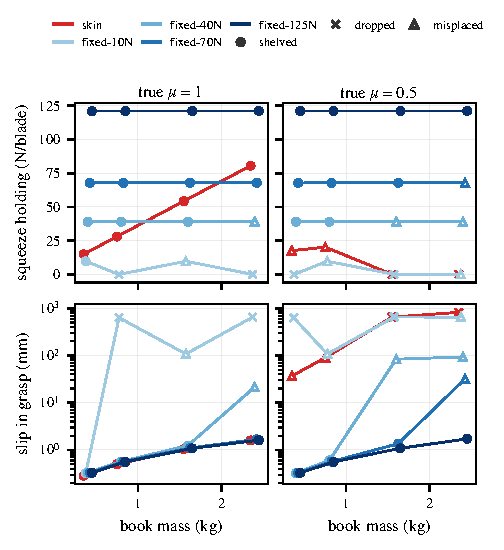
\includegraphics[width=\columnwidth]{fig_ablation.pdf}
\caption{Ablation, 40 runs: squeeze while holding (top) and the book's slip in the grasp until set-down (bottom) against book mass, for the true friction $\mu=1$ (left) and $\mu=0.5$ (right). Filled markers: shelved; open: misplaced ($\triangle$), dropped ($\times$). The skin controller (red) assumes $\hat\mu=1$.}
\label{fig:abl}
\end{figure}



%==============================================================================
\section{Limitations}\label{sec:lim}
\begin{itemize}
\item \textbf{The sensor is not modelled.} The panel shows what the model computes, on its $5\times7$ grid, at an
assumed 20\,Hz, without noise, drift or hysteresis. Calibrating the real skin's output against these quantities is
open work, as are its resolution and rate.
\item \textbf{Material values are placeholders.} $E=1$\,MPa, $\nu=0.45$ (real PDMS: $\approx$0.49, which makes the
confined layer several times stiffer in compression and leaves shear unchanged), $\tau_d=1$\,ms, $\mu=1$; all are
arguments of \code{make\_blade\_assets.py}. Deformations are micrometres either way (Fig.~\ref{fig:run}).
\item \textbf{Friction} is Coulomb with one $\mu$, no static/kinetic difference, and residual creep
($\approx$0.02--0.05\,mm/s under the book's twist) after raising MuJoCo's \code{impratio} to 100. Load sharing among
cells depends on the contact softness, so read the maps qualitatively; net forces are exact.
\item \textbf{The task is scripted}: hand-tuned thresholds, known shelf and book poses (no perception), one book
geometry, and every book rigid (its cover compliance is the contact softness).
\end{itemize}

{\footnotesize
\begin{thebibliography}{10}\setlength{\itemsep}{0pt}
\bibitem{todorov2012mujoco} E.~Todorov, T.~Erez, Y.~Tassa, ``MuJoCo: A physics engine for model-based control,''
\emph{IROS}, 2012.
\bibitem{todorov2014convex} E.~Todorov, ``Convex and analytically-invertible dynamics with contacts and
constraints: Theory and implementation in MuJoCo,'' \emph{ICRA}, 2014.
\bibitem{mujocodocs} MuJoCo 3.17 documentation: \emph{Computation} (soft constraints, integrators) and
\emph{Modeling: Deformable objects}, \url{https://mujoco.readthedocs.io}, 2026.
\bibitem{johnson1985} K.~L.~Johnson, \emph{Contact Mechanics}, Cambridge Univ. Press, 1985.
\bibitem{shull2002} K.~R.~Shull, ``Contact mechanics and the adhesion of soft solids,'' \emph{Mater. Sci. Eng. R},
36:1--45, 2002.
\bibitem{johnston2014} I.~D.~Johnston, D.~K.~McCluskey, C.~K.~L.~Tan, M.~C.~Tracey, ``Mechanical characterization
of bulk Sylgard 184 for microfluidics and microengineering,'' \emph{J. Micromech. Microeng.}, 24:035017, 2014.
\bibitem{goyal1991} S.~Goyal, A.~Ruina, J.~Papadopoulos, ``Planar sliding with dry friction, Part 1: Limit surface
and moment function,'' \emph{Wear}, 143:307--330, 1991.
\bibitem{howe1996} R.~D.~Howe, M.~R.~Cutkosky, ``Practical force-motion models for sliding manipulation,''
\emph{IJRR}, 15(6):557--572, 1996.
\bibitem{wampler1986} C.~W.~Wampler, ``Manipulator inverse kinematic solutions based on vector formulations and
damped least-squares methods,'' \emph{IEEE Trans. SMC}, 16(1):93--101, 1986.
\bibitem{romano2011} J.~M.~Romano, K.~Hsiao, G.~Niemeyer, S.~Chitta, K.~J.~Kuchenbecker, ``Human-inspired robotic
grasp control with tactile sensing,'' \emph{IEEE Trans. Robotics}, 27(6):1067--1079, 2011.
\bibitem{dong2017} S.~Dong, W.~Yuan, E.~H.~Adelson, ``Improved GelSight tactile sensor for measuring geometry and
slip,'' \emph{IROS}, 2017.
\end{thebibliography}}
\end{document}
